\documentclass[11pt]{article}
\usepackage[a4paper,pdftex]{geometry}
\setlength{\oddsidemargin}{5mm}
\setlength{\evensidemargin}{5mm}
\usepackage[english]{babel}
\usepackage{amsmath,amsfonts,amsthm,amssymb}
\usepackage{graphicx}
\usepackage{fancyhdr}
\pagestyle{fancy}
\usepackage{subfig}
\usepackage{wrapfig}
\usepackage{comment}
\usepackage{url}
\urlstyle{same}

% Page numbering
\lhead{Dutch Nao Team - Team Description for Robocup 2012}
\rhead{page \thepage/5}
\cfoot{}
\rfoot{\thepage}

% TITLE FORMAT
\newcommand{\HRule}[1]{\rule{\linewidth}{#1}}

\makeatletter
\def\printtitle{
    {\centering \@title\par}}
\makeatother									

\makeatletter
\def\printauthor{
    {\centering \large \@author}}
\makeatother

% TITLE
\title{
\HRule{0.5pt} \\
\LARGE \textbf{\textsc{Dutch Nao Team}}\\[0.5cm]
\normalsize \textsc{Team Description for Iran Open 2012 - Tehran, Iran}\\
\texttt{http://www.dutchnaoteam.nl}
\normalsize
\HRule{2pt}\\ [0.5cm]
\normalsize
\today\\ [0.5cm]
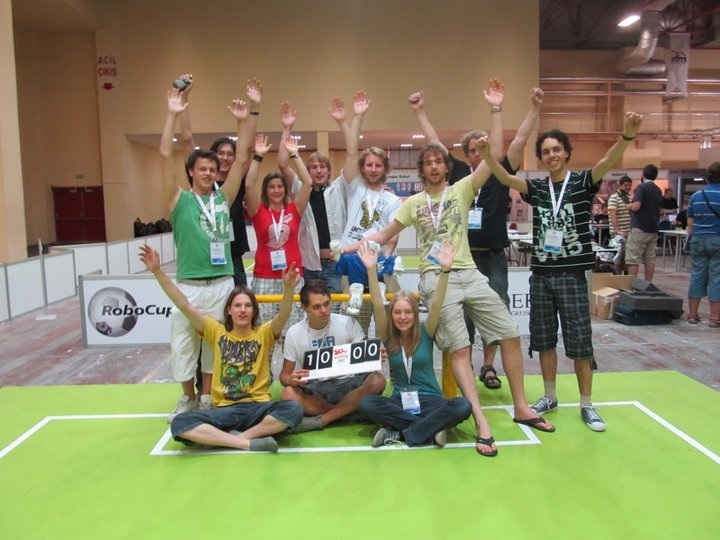
\includegraphics[width=0.8\textwidth]{team.jpg}
}

\author{
{\small Duncan ten Velthuis\footnote{Coordinator}, Camiel Verschoor, Auke Wiggers\footnote{Vice Coordinators} \\
Michael Cabot, Anna Keune, Sander Nugteren, Hendrik van Egmond, \\
Tim van Rossum, Hessel van der Molen, Richard Rozeboom\footnote{Senior members} \\
Inge Becht, Maarten de Jonge, Richard Pronk,
Chiel Kooijman, Roman Slaap \\
and Arnoud Visser\footnote{Supervisor}}\\ [0.2cm]
%\\
Dutch Nao Team\\
Faculty of Science\\
Universiteit van Amsterdam\\
\texttt{dutchnaoteam@googlegroups.com} \\
}


% BEGIN DOCUMENT
\begin{document}
\thispagestyle{empty}

% TITLE PAGE
\printtitle									
\vfill
\printauthor
\newpage
\setcounter{page}{1}
\normalsize
% CONTENT
\section{Introduction}
The Dutch Nao Team consists of Artificial Intelligence (AI) Bachelor and Master Students, supported by a senior staff-member.
%The Dutch Nao Team is the continuation of the Dutch Aibo Team; a cooperation of several Dutch universities who were active in the predecessor of the Standard Platform League \cite{AIBOTeam2006, AIBOTeam2005, AIBOTeam2004}. The Dutch Aibo Team has been successful, both in the competition and with a number of publications \cite{ArnoudJurgen2009, RoboticDog2008, Visser2006, ColorLearning2006, Localization2006, Perception2005}. The Dutch Aibo Team has the tradition to published their source-code online including a technical report about the innovations \cite{Visser2006, Sturm2005, Oomes2005}. 
The Dutch Nao Team debuted in the Standard Platform League (SPL) competition at the German Open 2010 \cite{DutchNaoTeamTDP2010}. The same year the first research paper about the Nao was published \cite{vanDerMey2011}. 
In 2011 the Dutch Nao Team made its breakthrough by qualifying for the World RoboCup in Istanbul \cite{DutchNaoTeamTDP2011}.

This year six new students will participate in the team in order to guarantee the continuity of the team. 
\begin{comment}
%moved to frontpage
The current team consists of the following persons:
\begin{description}
\item[Supervisor:] Dr. Arnoud Visser
\item[Coordinator:] Duncan ten Velthuis
\item[Vice Coordinators:] Camiel Verschoor and Auke Wiggers
\item[Senior Students:] Michael Cabot, Anna Keune, Sander Nugteren, Hendrik van Egmond, Tim van Rossum, Hessel van der Molen, Richard Rozeboom
\item[Students:] Inge Becht, Maarten de Jonge, Richard Pronk, Chiel Kooijman and Roman Slaap
\end{description}
\end{comment}
This year the Dutch Nao Team is planning to participate in the competition of the following opens:
\begin{itemize}
\item RoBOW 12.1 (February 2012)
\item German Open (29-03-2012 until 01-04-2012)
\item Iran Open (03-04-2012 until 07-04-2012)
\item Dutch Open demonstration (25-04-2012 until 29-04-2012)
\end{itemize}
\begin{comment}
Next to participating in competitions, the Dutch Nao Team will also be active at the Dutch Open in Eindhoven (25-04-2012 until 29-04-2012) with the following activities:
\begin{itemize}
\item SPL demonstration
\item Dutch Nao Users Day (workshop organized by Aldebaran)
\item RoboCup Junior 
\end{itemize}
\end{comment}
\section{Relevant Achievements and Publications}
%In 2010 the Universiteit van Amsterdam bought two academic editions of the Nao and participated for the first time in the Standard Platform League at the German Open \cite{DutchNaoTeamTDP2010}. 
The Dutch Nao Team is a continuation of the Dutch Aibo Team, which participated at three competitions and published on several occasions\footnote{See for an overview \url{http://www.dutchnaoteam.nl/index.php/publications/}}. 
%Since the Dutch Nao Team qualified for the RoboCup in Istanbul, the Universiteit van Amsterdam is now also in the possession of five v3.3 Nao robots. 
The Dutch Nao Team participated both at the Mediterranean Open 2011 and in the Iran Open 2011.  In Istanbul 2011 the team became second in the first round and survived the elimination round in a penalty shoot-out against SPQR-Chili, resulting in a top 16 position. At the Mediterranean Open Workshop on RoboCup Research a presentation about "RoboTag with a humanoid robot" was given.
At the RoboCup Iran Open Symposium the paper 'An Experimental Comparison of Mapping Methods, the Gutmann dataset' was published \cite{Visser2011rios}. A summary of this study was presented at the Research Challenge in Istanbul.
\subsection*{Support}
The Universiteit van Amsterdam has been active in the RoboCup since Paris 1998. The university has been participated in several leagues (Windmill Wanderers, Clockwork Orange, UvA TriLearn, UvA Rescue, Dutch Aibo Team, Amsterdam Oxford Joint Rescue Forces).
The Institute of Informatics supports the team with a fully equiped robot lab (large enough for the Standard Platform League soccer field) and the usage of two academic Nao robots and a package of five v3.3 Nao robots.
When the Dutch Nao Team qualifies for Mexico 2012, the Univerisiteit van Amsterdam will support us with new v4.0 Nao robots.
\section{Research}
%As a junior team, the educational aspect is important. 
The main focus of the Universiteit van Amsterdam is the combination of Artificial Intelligence and Robotics. The RoboCup initiative provides the team the opportunity to acquire various abilities of many aspects within robotics.
Research and education will be combined in the studies performed to graduate at our university. The shared goal is to establish a base code build in Python with a focus on motion, vision and localization. 
Python is a general-purpose high-level programming language whose design philosophy emphasizes code readability. Python aims to combine remarkable power with very clear syntax, and its standard library is large and comprehensive. 
Python is the brainchild of an alumnus of the Universiteit van Amsterdam and was built at the Science Park where our university is located. 
The Dutch Nao Team will subsequently increase the efficiency of its base code and will optimize it in the years to come. 
The Dutch Nao Team believes in open source, therefore, the project has been made available for the RoboCup community \cite{DutchNaoTeamTechReport2011}.
\subsection{Vision with C++}
This year the Dutch Nao Team started writing C++ vision modules, which can be called from Python. C++ will make the code faster and is a great investment for future projects. For now, Python is the base of the project and C++ a performance gain in the vision modules, where time is a crucial factor.

One of the recent developments towards vision in C++ is an improved ball-tracking algorithm. The previous implementation took the mean of all red pixels in the image. However, the new implementation locates the ball correctly using Hough transformation on a tresholded image. Although this is a heavier operation than the previous implemented Python code, this will be compensated by the benefit of the speed of C++. The current speed is comparable to our previous implementation (20 milliseconds against 25 milliseconds). Due to the improvement, the Nao robot will not detect all objects that have the correct hue of red, but will only detect objects that have a spherical characteristic as well, which was severely lacking in the previous implementation.
\begin{figure}[!ht]
  \centering
  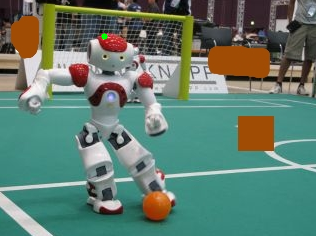
\includegraphics[width=0.4\textwidth]{bal2.png}
  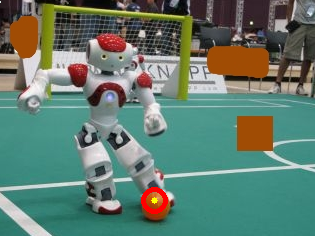
\includegraphics[width=0.4\textwidth]{bal.png}
  \caption{Left: Previous balltracking algorithm, the green dots indicates found ball location. Right: Improved vision module using Hough transform and C++.}
\label{fig:balls}
\end{figure}
\begin{wrapfigure}{r}{30mm}
  \begin{center}
    \vspace{0.5cm}
    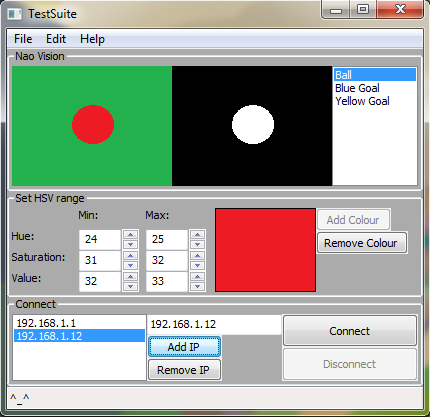
\includegraphics[width=0.3\textwidth]{testsuite.png}
  \end{center}
\end{wrapfigure}
\subsection{Test Suite}
During previous competitions calibration was time consuming. One of the goals of the test suite is to build a user-friendly interface that allows us to quickly calibrate the Nao robots for our vision applications. Besides calibration, the Test-Suite will also enable the team to easier view, edit, read and control our code running on the Nao robot. It will also provide the possibility to show self-localization results graphically.
The back-end of the test suite (also written in Python) will consist of a complete full-duplex communication system, which will enable sending, writing and reading of variables, data and files in real-time.
\subsection{Communication and Planning}
The Nao robots will communicate using a zeroconf protocol. The  communication between Nao robots will be kept to a minimum. The players will only act different from their originial behaviour, when a conflict is detected. For example, when two robots see the ball, only the closest robot will try to intercept it, while the behaviour of the other will be overridden. Together with localization and Nao robot recognition, a tactical behaviour can be implemented. For instance, assisting other Nao robots in an attacking state or defensive state.
\subsection{Localization}
For localization the Dutch Nao Team researches multiple methods: Dynamic Tree Localization, a Kalman Filter and a Particle filter. 
Dynamic Tree Localization \cite{vdMolen2011} splits the field recursively into blocks. Each block holds a probability that a Nao robot is in this block. 
Besides a probability, a block contains a list with the distance (a range) and the angle (also a range) towards each possible observable feature. 
As features, the goals and line crossings will be used. Children of a block which hold a probability lower than a certain threshold are removed.
Is the probability in a block higher than an another threshold, then the block is split. In this way it is possible to maintain a belief over all possible locations without the need to (re)sample.
It is assumed that such a tree-like structure results in a method with a lower computational complexity compared to other approaches, while it does hold the possibility to create a complex belief. 
Dynamic Tree Localization can also estimate the location of the Nao robot in a accurate way; is robust against noisy data; can handle kidnapping; and does not have to keep track of previous observed observations \cite{vdMolen2011}.
This localization algorithm will be compared against standard reference algorithms such as a Kalman or Particle filter. 
% This gives the possibility to compare both systems and to further our research. The latest addition to the the rules, same coloured goals, make it important to have a robust localization system.
\subsection{Simulator}
The 3D robot simulation environment (USARSim) is extended with the possibility to reproduce the appearance and the dynamics of generic legged robots and especially a humanoid Nao robot. USARSim is based on the Unreal Engine, which provides facilities for good quality rendering, physics simulation, networking, highly versatile scripting language and a powerful visual editor. Building a realistic simulator implies that interaction models are needed which replicate the dynamics of a walking robot with many body contacts, while maintaining a fast frame rate. Several approximations have been tried, and the performance evaluated. This extension could have a wide application range, which allows people to develop and experiment typical robotic tasks at home, without requiring a real robot.
\begin{figure}[!ht]
\centering
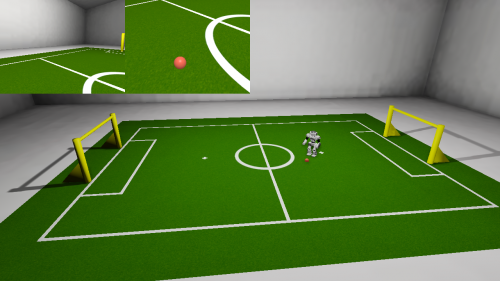
\includegraphics[width = 0.75\textwidth]{sim2012.png} % 0.5 is also OK, but I like to have the conclusion
\caption{A simulation of a Nao robot in USARSIM environment}
\end{figure}
The development of this open source simulation is not only valuable inside the Standard Platform League, but should also be interesting for the Soccer Simulation League and the @ Home League. Outside the RoboCup community this simulation could be valuable for Human-Robot Interaction research.
\subsection{Motion Control}
The motions of last year will be improved by making them more robust and secure. Examples of these motions are the keeper dive, the heelkick and the sidekicks. A few of those innovations are demonstrated in the 2012 Qualification video\footnote{See for a larger overview \url{http://www.dutchnaoteam.nl/index.php/media/movies}}. Thanks to the development of a realistic Nao simulation, it is easier to develop new motions, either manually or by supervised learning.
\section{Conclusion}
The Dutch Nao Team will continue using its unique Python based approach and extend it with C++ based modules. This year we hope to show the benefits of a global localization technique as the Dynamic Tree Localization algorithm and improve our behaviour modules based on this additional information.
Coordination between the robots will result in joint behaviors as attacking, defending or even passing.
\bibliographystyle{plain}
\bibliography{references} 
\end{document}
% END DOCUMENT